\documentclass[a4paper,11pt]{article}

\usepackage[margin=2.5cm]{geometry}
\usepackage{tikz}
\usetikzlibrary{shapes.geometric, arrows.meta, positioning}
\usepackage{algorithm}
\usepackage{algpseudocode}

\begin{document}

\section*{Tugas 1: Algoritma, Pseudocode, dan Flowchart Penentuan Grade Siswa}

\subsection*{Deskripsi Masalah}
Seorang guru ingin menentukan nilai huruf (grade) seorang siswa berdasarkan nilai ujiannya (skala 0--100), dengan ketentuan:
\begin{itemize}
    \item Nilai $\geq 85$ $\rightarrow$ A
    \item Nilai $70-84$ $\rightarrow$ B
    \item Nilai $55-69$ $\rightarrow$ C
    \item Nilai $< 55$ $\rightarrow$ D
\end{itemize}

\subsection*{Algoritma Deskriptif}
\begin{enumerate}
    \item Mulai.
    \item Masukkan nilai ujian siswa.
    \item Jika nilai $\geq 85$, maka grade = A.
    \item Jika tidak, jika nilai $\geq 70$, maka grade = B.
    \item Jika tidak, jika nilai $\geq 55$, maka grade = C.
    \item Jika tidak, maka grade = D.
    \item Cetak grade.
    \item Selesai.
\end{enumerate}

\subsection*{Pseudocode}
\begin{algorithm}[h]
\caption{Penentuan Grade Siswa}
\begin{algorithmic}[1]
\State \textbf{Input:} nilai
\If{nilai $\geq 85$}
    \State grade $\gets$ "A"
\ElsIf{nilai $\geq 70$}
    \State grade $\gets$ "B"
\ElsIf{nilai $\geq 55$}
    \State grade $\gets$ "C"
\Else
    \State grade $\gets$ "D"
\EndIf
\State \textbf{Output:} grade
\end{algorithmic}
\end{algorithm}

\subsection*{Flowchart}

\begin{center}
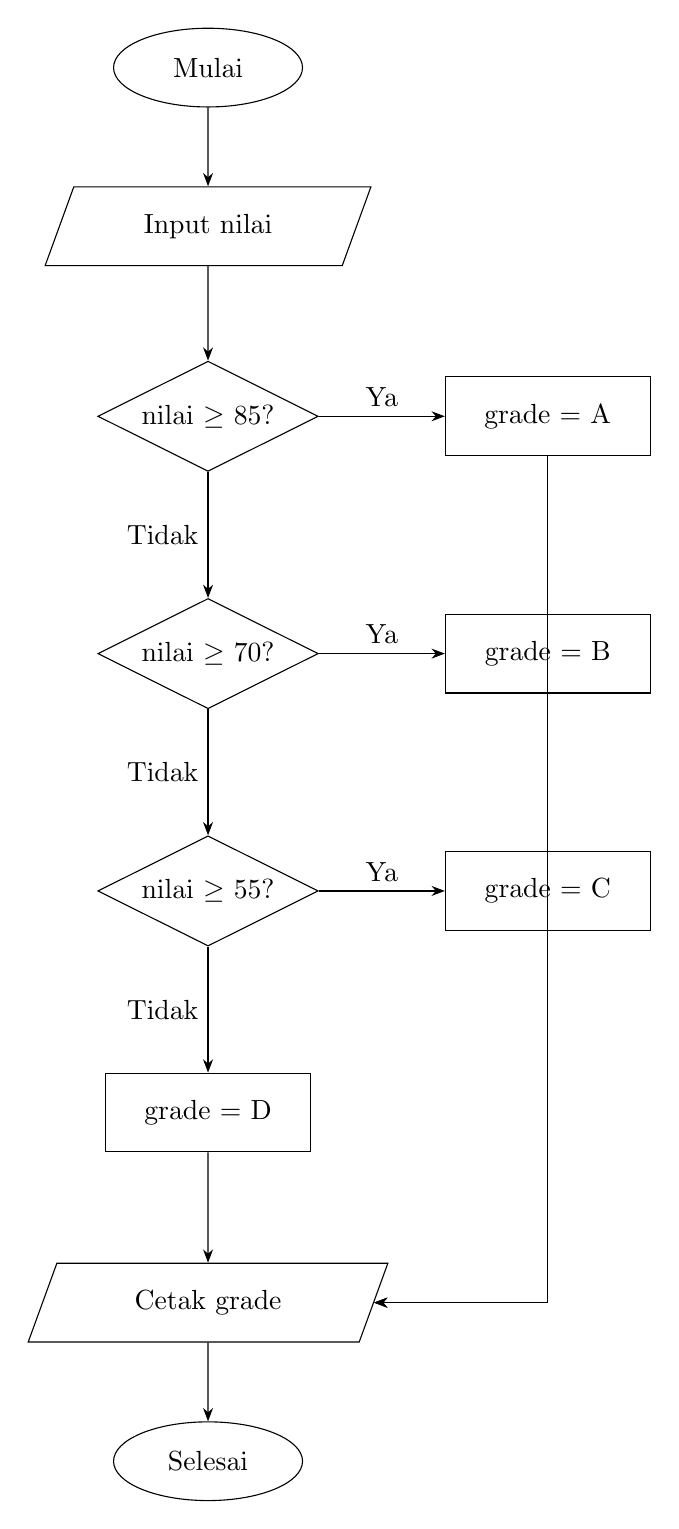
\begin{tikzpicture}[
    node distance=1cm and 1.6cm,
    terminator/.style={ellipse, draw, minimum width=2.4cm, minimum height=1cm, align=center},
    io/.style={trapezium, trapezium left angle=70, trapezium right angle=110, draw, minimum width=2.6cm, minimum height=1cm, align=center},
    process/.style={rectangle, draw, minimum width=2.6cm, minimum height=1cm, align=center},
    decision/.style={diamond, draw, aspect=2, minimum width=2.8cm, minimum height=1.4cm, align=center, inner sep=1pt},
    arrow/.style={-{Stealth}}
]

\node[terminator] (start) {Mulai};
\node[io, below=of start] (input) {Input nilai};
\node[decision, below=1.2cm of input] (dec1) {nilai $\geq$ 85?};
\node[process, right=of dec1] (gA) {grade = A};

\node[decision, below=1.6cm of dec1] (dec2) {nilai $\geq$ 70?};
\node[process, right=of dec2] (gB) {grade = B};

\node[decision, below=1.6cm of dec2] (dec3) {nilai $\geq$ 55?};
\node[process, right=of dec3] (gC) {grade = C};

\node[process, below=1.6cm of dec3] (gD) {grade = D};

\node[io, below=1.4cm of gD] (output) {Cetak grade};
\node[terminator, below=of output] (end) {Selesai};

\draw[arrow] (start) -- (input);
\draw[arrow] (input) -- (dec1);

\draw[arrow] (dec1) -- node[above]{Ya} (gA);
\draw[arrow] (dec1) -- node[left]{Tidak} (dec2);

\draw[arrow] (dec2) -- node[above]{Ya} (gB);
\draw[arrow] (dec2) -- node[left]{Tidak} (dec3);

\draw[arrow] (dec3) -- node[above]{Ya} (gC);
\draw[arrow] (dec3) -- node[left]{Tidak} (gD);

\draw[arrow] (gA) |- (output);
\draw[arrow] (gB) |- (output);
\draw[arrow] (gC) |- (output);
\draw[arrow] (gD) -- (output);

\draw[arrow] (output) -- (end);

\end{tikzpicture}
\end{center}

\end{document}
